Cytoscape~可以读取以下格式的网络或路径文件:
\begin{itemize}
\item Simple interaction file (SIF or .sif format) 
\item Graph Markup Language (GML or .gml format) 
\item XGMML (extensible graph markup and modelling language). 
\item SBML 
\item BioPAX 
\item PSI-MI Level 1 and 2.5 
\item Delimited text 
\item Excel Workbook (.xls) 
\end{itemize}

SIF~格式的文件只有节点和相互作用,而其它的格式都可以存储网络布局信息,还可以跟其它的网络软件和数据源交换数据。SIF~文件通常用于在新建网络时导入相互作用,因为用文本编辑器和电子表格软件能很方便的创建这种格式的文件。在导入了相互作用,应用了某种网络布局后,就可以将网络存为GML或XGMML格式,从而能去其它系统交换数据。所有的这些格式(Excel例外)都是文本文件,用普通的文本编辑器就能编辑和查看这些文件。


\section{SIF~格式}
这种简单的格式可以很方便地用于从相互作用列表构建网络。利用这种格式,还能很方便的把小网络组合在一起,或是在现有的数据中添加新的相互作用。但这种格式的缺点也是显而易见的,其中不包含布局信息,这使得Cytoscape不得不在每次加载网络时都重新计算网络的布局。

SIF~文件中的每行都由起点、相互作用类型(或边的类型)和一个或若干个重点构成。
\begin{verbatim}
nodeA <relationship type> nodeB
nodeC <relationship type> nodeA
nodeD <relationship type> nodeE nodeF nodeB
nodeG
...
nodeY <relationship type> nodeZ
\end{verbatim}

下面是一个具体的例子:
 \begin{verbatim}
node1 typeA node2
node2 typeB node3 node4 node5
node0
\end{verbatim}

第一行是两个节点,node1和node2,以及两点间的typeA型的相互关系。第二行加入了三个新节点,node3~、\linebreak node4~和~node5,这一行中的node2跟第一行中的node2是同一个节点。第二行还设定了三条起点相同且类型也相同的相互作用。第三行说明了如何引入孤立的节点。 This form is not needed for nodes that do have relationships, since the specification of the relationship implicitly identifies the nodes as well. 

重复的条目被忽略。两个点之间的多条相互作用必须是不同的类型。例如,下面的node1和node2之间就有两条边,但类型分别是xx和yy。
\begin{verbatim}
node1 xx node2
node1 xx node2
node1 yy node2
\end{verbatim}

节点的自相互作用是允许的:
\begin{verbatim}
node1 xx node1
\end{verbatim}

 Every node and edge in Cytoscape has an identifying name, most commonly used with the node and edge data attribute structures. Node names must be unique, as identically named nodes will be treated as identical nodes. The name of each node will be the name in this file by default (unless another string is mapped to display on the node using the visual mapper). This is discussed in the section on visual styles. The name of each edge will be formed from the name of the source and target nodes plus the interaction type: for example, sourceName (edgeType) targetName. 


 The tag $<$relationship type$>$ can be any string. Whole words or concatenated words may be used to define types of relationships, e.g. geneFusion, cogInference, pullsDown, activates, degrades, inactivates, inhibits, phosphorylates, upRegulates, etc. 


 Some common interaction types used in the Systems Biology community are as follows: 
\begin{verbatim}
  pp .................. protein – protein interaction
  pd .................. protein -> DNA   
  (e.g. transcription factor binding upstream of a regulating gene.)

\end{verbatim}


 Some less common interaction types used are: 
\begin{verbatim}
  pr .................. protein -> reaction
  rc .................. reaction -> compound
  cr .................. compound -> reaction
  gl .................. genetic lethal relationship
  pm .................. protein-metabolite interaction
  mp .................. metabolite-protein interaction

\end{verbatim}


\textbf{Delimiters}

Whitespace (space or tab) is used to delimit the names in the simple interaction file format. However, in some cases spaces are desired in a node name or edge type. The standard is that, if the file contains any tab characters, then tabs are used to delimit the fields and spaces are considered part of the name. If the file contains no tabs, then any spaces are delimiters that separate names (and names cannot contain spaces). 

 If your network unexpectedly contains no edges and node names that look like edge names, it probably means your file contains a stray tab that's fooling the parser. On the other hand, if your network has nodes whose names are half of a full name, then you probably meant to use tabs to separate node names with spaces. 

 Networks in simple interactions format are often stored in files with a .sif extension, and Cytoscape recognizes this extension when browsing a directory for files of this type. 

\section{GML Format}
 In contrast to SIF, GML is a rich graph format language supported by many other network visualization packages. The GML file format specification is available at: \url{http://www.infosun.fmi.uni-passau.de/Graphlet/GML/}

 It is generally not necessary to modify the content of a GML file directly. Once a network is built in SIF format and then laid out, the layout is preserved by saving to and loading from GML. Visual attributes specified in a GML file will result in a new visual style named Filename.style when that GML file is loaded. 

\section{XGMML Format}


 XGMML is the XML evolution of GML and is based on the GML definition. In addition to network data, XGMML contains node/edge/network attributes. The XGMML file format specification is available at: 


 \url{http://www.cs.rpi.edu/~puninj/XGMML/}


 XGMML is now preferred to GML because it offers the flexibility associated with all XML document types. If you're unsure about which to use, choose XGMML. 


 
\section{SBML (Systems Biology Markup Language) Format}


 The Systems Biology Markup Language (SBML) is an XML format to describe biochemical networks. SBML file format specification is available at: 


 \url{http://sbml.org/documents/}


 
\section{BioPAX (Biological PAthways eXchange) Format}


 BioPAX is an OWL (Web Ontology Language) document designed to exchange biological pathways data. The complete set of documents for this format is available at: 


 \url{http://www.biopax.org/index.html}


 
\section{PSI-MI Format}


 The PSI-MI format is a data exchange format for protein-protein interactions. It is an XML format used to describe PPI and associated data. PSI-MI XML format specification is available at: 


 \url{http://psidev.sourceforge.net/mi/xml/doc/user/}


 
\section{Delimited Text Table and Excel Workbook}


 Cytoscape has native support for Microsoft Excel files (.xls) and delimited text files. The tables in these files can have network data and edge attributes. Users can specify columns containg source nodes, target nodes, interaction types, and edge attributes during file import. Some of the other network analysis tools, such as igraph (\url{http://cneurocvs.rmki.kfki.hu/igraph/}), has feature to export graph as simple text files. Cytoscape can read these text files and build networks from them. For more detail, please read the Import Free-Format Tables section section of the Creating Networks chapter. 

\centerline{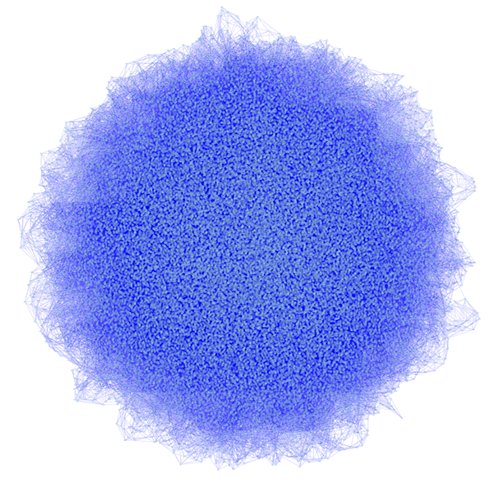
\includegraphics[width=.7\textwidth]{images/huge_network_igraph.png}}

 \textbf{Network generated by igraph's Watts-Strogatz small-world model (50k nodes and 250k esges) visualized by Cytoscape:}
 You can import networks created by other applications using this Table Import feature. 
 
\section{Node Naming Issues in Cytoscape}

 Typically, genes are represented by nodes, and interactions (or other biological relationships) are represented by edges between nodes. For compactness, a gene also represents its corresponding protein. Nodes may also be used to represent compounds and reactions (or anything else) instead of genes. 

 If a network of genes or proteins is to be integrated with Gene Ontology (GO) annotation or gene expression data, the gene names must exactly match the names specified in the other data files. We strongly encourage naming genes and proteins by their systematic ORF name or standard accession number; common names may be displayed on the screen for ease of interpretation, so long as these are available to the program in the annotation directory or in a node attribute file. Cytoscape ships with all yeast ORF-to-common name mappings in a synonym table within the annotation/ directory. Other organisms will be supported in the future. 

 Why do we recommend using standard gene names? All of the external data formats recognized by Cytoscape provide data associated with particular names of particular objects. For example, a network of protein-protein interactions would list the names of the proteins, and the attribute and expression data would likewise be indexed by the name of the object. 

 The problem is in connecting data from different data sources that don't necessarily use the same name for the same object. For example, genes are commonly referred to by different names, including a formal ``location on the chromosome'' identifier and one or more common names that are used by ordinary researchers when talking about that gene. Additionally, database identifiers from every database where the gene is stored may be used to refer to a gene (e.g. protein accession numbers from Swiss-Prot). If one data source uses the formal name while a different data source used a common name or identifier, then Cytoscape must figure out that these two different names really refer to the same biological entity. 

 Cytoscape has two strategies for dealing with this naming issue, one simple and one more complex. The simple strategy is to assume that every data source uses the same set of names for every object. If this is the case, then Cytoscape can easily connect all of the different data sources. 


 To handle data sources with different sets of names, as is usually the case when manually integrating gene information from different sources, Cytoscape needs a data server that provides synonym information (see the chapter on Annotation). A synonym table gives a canonical name for each object in a given organism and one or more recognized synonyms for that object. Note that the synonym table itself defines which set of names are the ``canonical'' names. For example, in budding yeast, the ORF names are commonly used as the canonical names. 


 If a synonym server is available, then by default Cytoscape will convert every name that appears in a data file to the associated canonical name. Unrecognized names will not be changed. This conversion of names to a common set allows Cytoscape to connect the genes present in different data sources, even if they have different names \^a€“ as long as those names are recognized by the synonym server. 


 For this to work, Cytoscape must also be provided with the species to which the objects belong, since the data server requires the species in order to uniquely identify the object referred to by a particular name. This is usually done in Cytoscape by specifying the species name on the command line with the \^a€“P option (cytoscape.sh -P ``defaultSpeciesName=Saccharomyces cerevisiae'') or by editing the properties (under Edit \^a†’ Preferences \^a†’ Properties...). 

 The automatic canonicalization of names can be turned off using the -P option (cytoscape.sh -P canonicalizeName=false'') or by editing the properties (under Edit \^a†’ Preferences \^a†’ Properties...). This canonicalization of names currently does not apply to expression data. Expression data should use the same names as the other data sources or use the canonical names as defined by the synonym table. 
